\documentclass[xcolor=dvipsnames]{beamer}
\usepackage[T1]{fontenc}
\usepackage[utf8]{inputenc}
\usepackage[english,slovak]{babel}

\usepackage{amsmath}
\usepackage{amsthm}
\usetheme{Pittsburgh}
\useoutertheme{shadow}

\usepackage{graphicx}
\usepackage{caption}
\usepackage{subcaption}

\usepackage[]{algorithm2e}
\usepackage{listings}
 \setbeamercovered{transparent}
 \usepackage{cuted}
\usepackage[export]{adjustbox}
\usepackage{mathtools}

\usepackage{lipsum}

\newcommand\Wider[2][3em]{%
\makebox[\linewidth][c]{%
  \begin{minipage}{\dimexpr\textwidth+#1\relax}
  \raggedright#2
  \end{minipage}%
  }%
}

%-------------------------------------------------------------------------------------
\title{\bf Deep learning}
\author{Michal CHOVANEC, PhD.}


%\setbeamertemplate{footline}[frame number]{}
\setbeamertemplate{navigation symbols}{}


\date[EURP]{\it May 2018}
\begin{document}

\begin{frame}
\titlepage
\centering{Faculty of Management Science and Informatics}
\end{frame}

\begin{frame}{\bf Stack game}

\begin{figure}
\centering
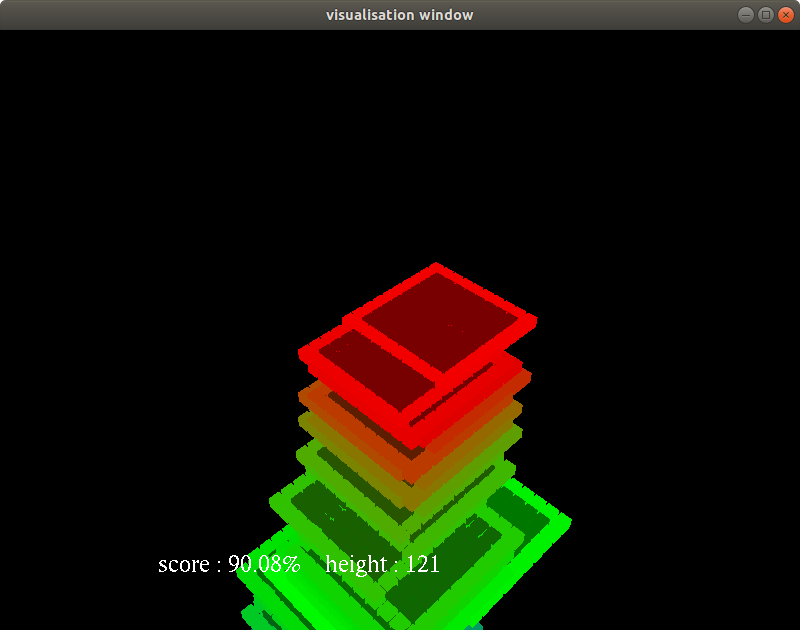
\includegraphics[scale=0.32]{stack.png}
\end{figure}

\end{frame}




\begin{frame}{\bf Stack game}

\begin{minipage}{.5\textwidth}

    \begin{figure}[htbp]
      \centering
      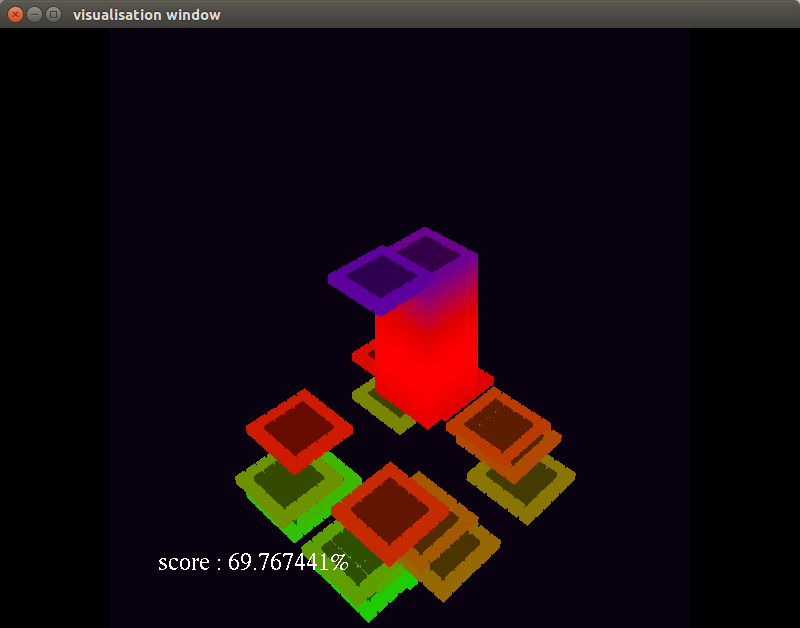
\includegraphics[scale=0.2]{stack_2.png}
    \end{figure}

\end{minipage}%
\begin{minipage}{.5\textwidth}

  \begin{itemize}
   \item build stack tower
   \item {\bf state}  : last + actual floor image [32x32x2]
   \item {\bf reward} : alignment rate $\langle 0, 1 \rangle$
  \end{itemize}

\end{minipage}

\end{frame}



\begin{frame}{\bf Neural network}

\begin{figure}[htbp]
  \centering
  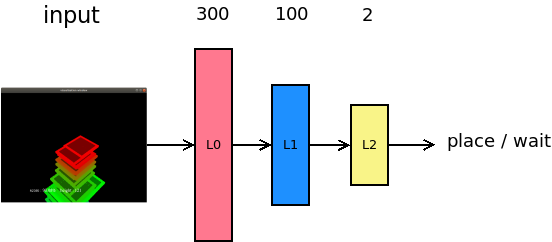
\includegraphics[scale=0.5]{dnn.png}
\end{figure}

\end{frame}

\begin{frame}{\bf Neural network, training}


\begin{minipage}{.5\textwidth}

\begin{figure}[htbp]
  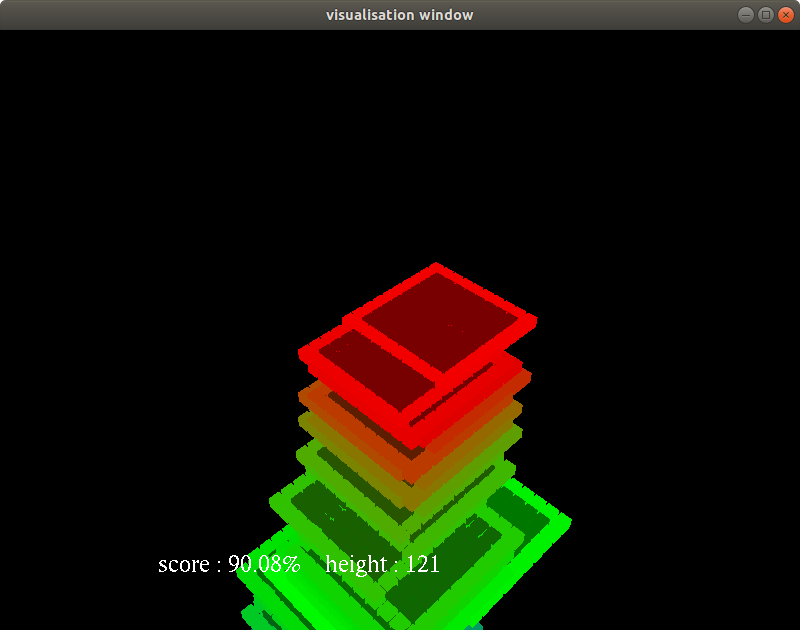
\includegraphics[scale=0.07]{tr_01.png}
  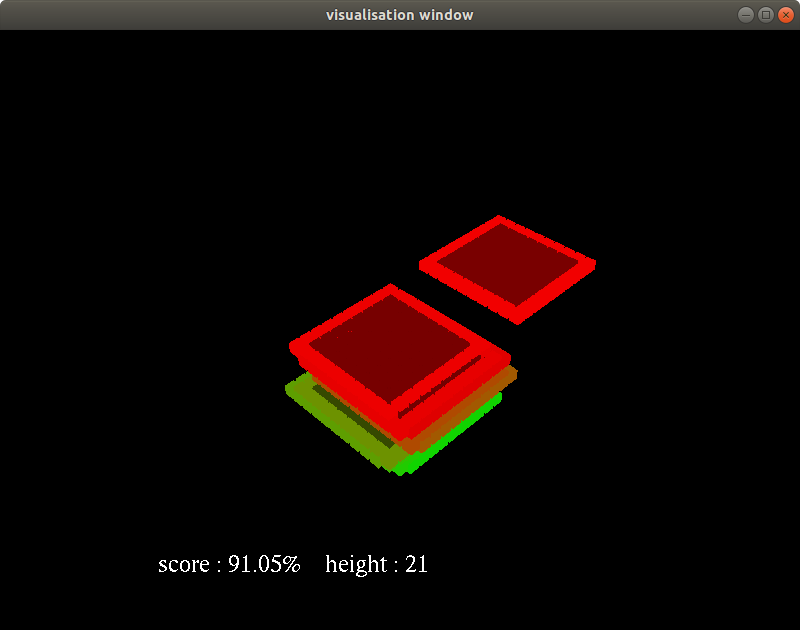
\includegraphics[scale=0.07]{tr_02.png}
  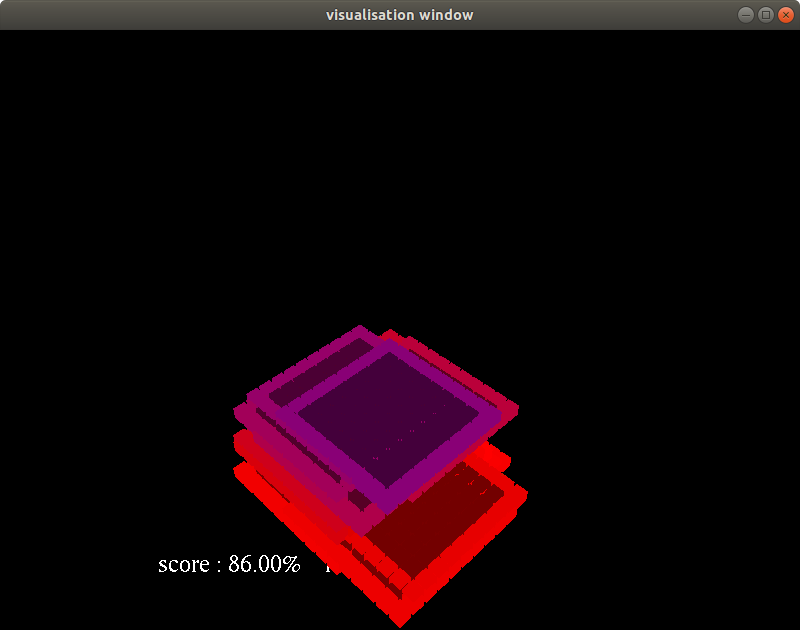
\includegraphics[scale=0.07]{tr_03.png}
  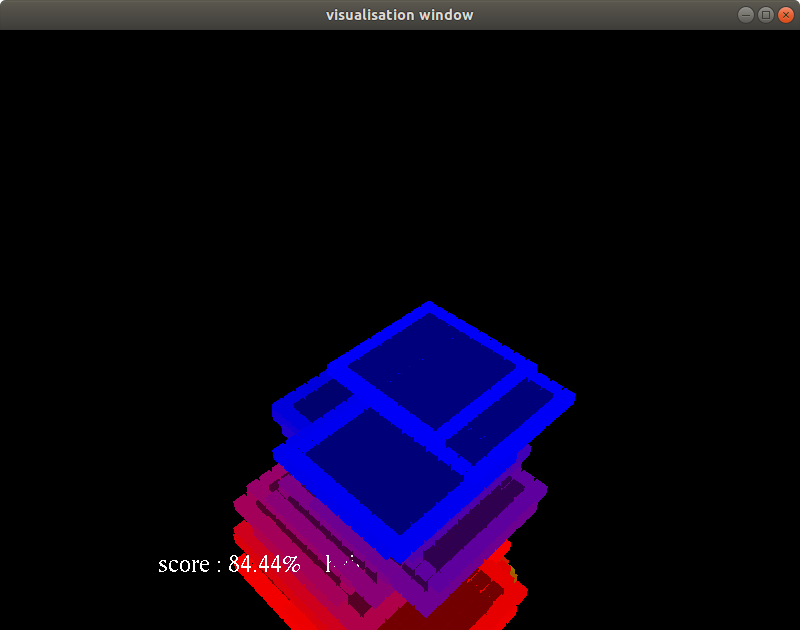
\includegraphics[scale=0.07]{tr_04.png}
  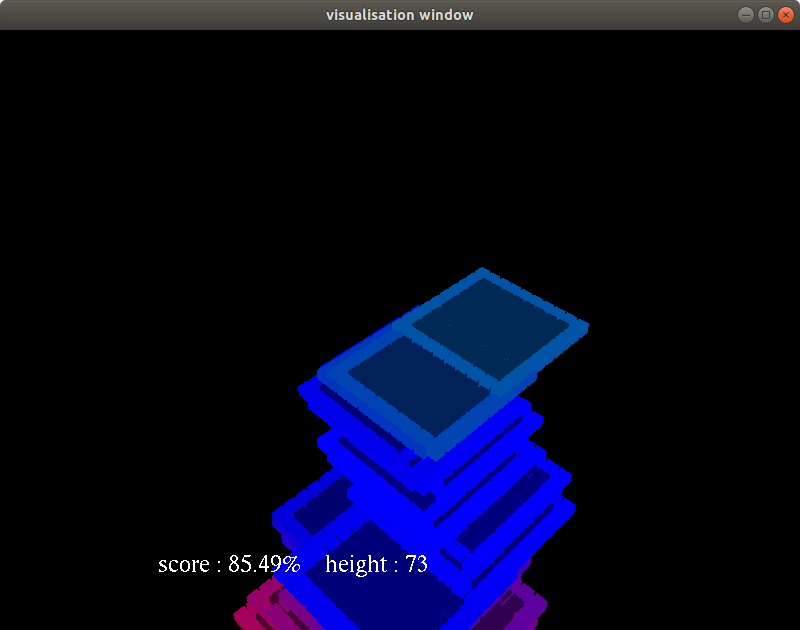
\includegraphics[scale=0.07]{tr_05.png}
  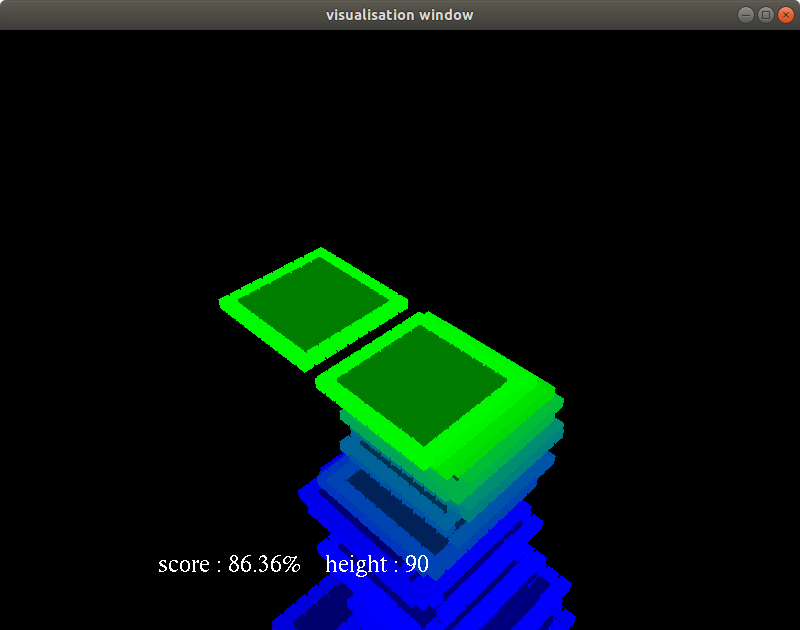
\includegraphics[scale=0.07]{tr_06.png}
\end{figure}

\end{minipage}%
\begin{minipage}{.5\textwidth}

  \begin{itemize}
    \item training set
    \item thousands of inputs and required outputs
    \item {\small \bf Error = required - obtained}
    \item learn neural network
  \end{itemize}

\end{minipage}

\end{frame}


\begin{frame}[fragile]
{\bf Neural network}


{\tiny
\begin{verbatim}
layer IO                   : [  20   20    2][   1    1    1][  20   20    2][    0     0]
layer AV POOLING           : [  20   20    2][   2    2    1][  10   10    2][    0     0]
layer FC                   : [   1    1  200][   1    1   64][   1    1   64][12800    64]
layer RELU                 : [   1    1   64][   1    1    1][   1    1   64][    0     0]
layer FC                   : [   1    1   64][   1    1    8][   1    1    8][  512     8]
layer RELU                 : [   1    1    8][   1    1    1][   1    1    8][    0     0]
layer FC                   : [   1    1    8][   1    1    2][   1    1    2][   16     2]
layer IO                   : [   1    1    2][   1    1    1][   1    1    2][    0     0]
\end{verbatim}
}

\end{frame}





%-------------------------------------------------------------------------------------
\begin{frame}{\bf Q\&A}


\begin{figure}[htbp]
  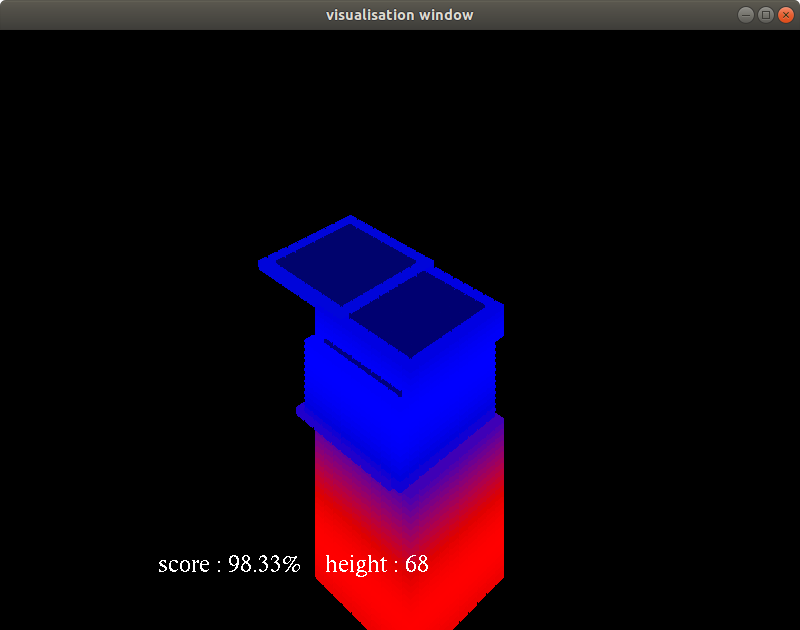
\includegraphics[scale=0.3]{final.png}
\end{figure}

\url{https://github.com/michalnand/machine\_learning\_course}

\centerline{michal.nand@gmail.com}

\end{frame}

\end{document}
